\section{BP神经网络}
\subsection{神经网络的构造与前向传播}
神经网络是由单个或多个神经元组成。下面是单个神经元的构造。
\begin{center}
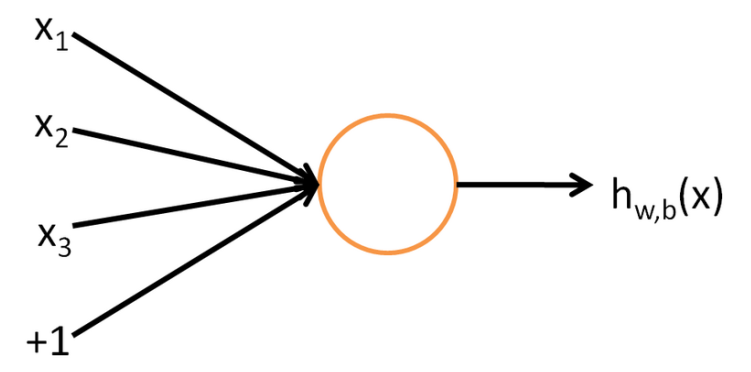
\includegraphics[scale=0.5]{../figures/NN1.png}\\
\textbf{图1}:神经元 
\end{center}
该神经元的输入由三个数据$x_1,x_2,x_3$以及偏置项(bias)+1组成,通过神经元后输出的表达式为
\begin{eqnarray}
h_{W,b}(x)=f(W^Tx+b)=f(\sum_{i=1}^3 W_ix_i+b)
\end{eqnarray}
其中$f$为激活函数。激活函数是为了将线性项$W^Tx$变换为非线性。在BP中,较常用的激活函数为sigmoid函数,其表达式如下
\begin{eqnarray}
f(z)=\frac{1}{1+\exp(-z)}
\end{eqnarray}
另外,令$b=w_0$,则可重新定义$W=(w_0,w_1,w_2,w_3)^T$,$x=(1,x_1,x_2,x_3)$,于是可将上式写为
\begin{eqnarray}
h_{W,b}(x)=f(W^Tx)
\end{eqnarray}
下面讨论神经网络。多个神经元可以组成一个层,多个层互相连接可以组成神经网络。其中,接受数据输入的层为输入层,数据计算后的数据的输出层,中间的层则称为隐含层。为下图是含有两个隐含层的神经网络。
\begin{center}
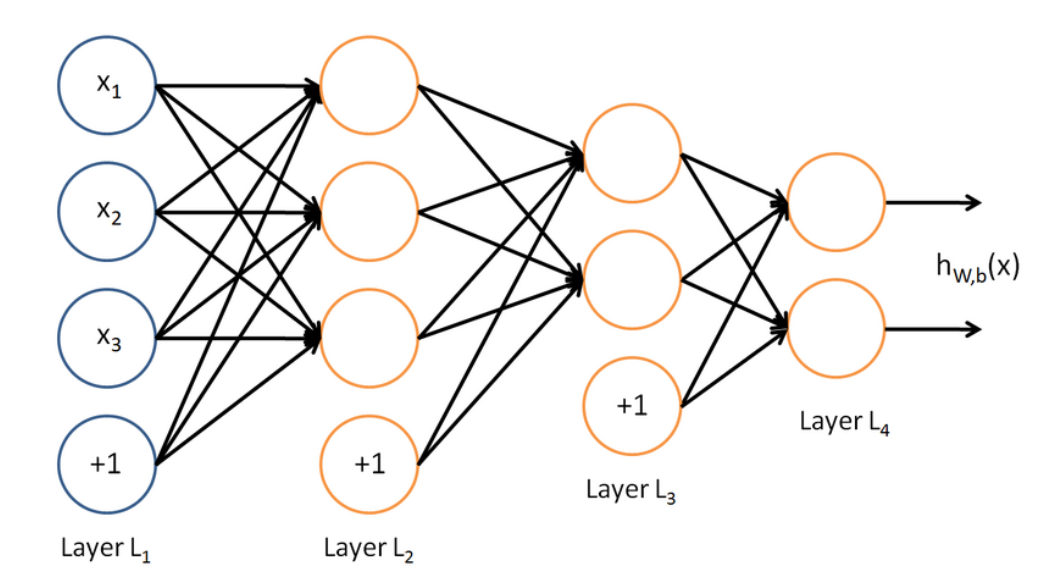
\includegraphics[scale=0.5]{../figures/NN2.png}\\
\textbf{图2}:含有两个隐含层的神经网络
\end{center}
如图,最左边的为输入层,即图中的Layer L1,最右边的为输出层,即图中的Layer L4,中间的所有层,即图中的Layer L2,Layer L3为隐含层。

我们用$n_l$来表示网络的层数,记第$i$层为$L_i$,于是输入层为$L_1$,输出层为$L_{n_l}$。由于神经网络可以有任意多的隐层以及隐藏神经元,则我们记$\samplet{W}{l}{ij}$为第$l$层第$j$单元以及第$l+1$层第$i$单元之间的连接权重,$\samplet{b}{l}{i	}$为第$L+1$层第$i$单元的偏执。我们用$\samplet{a}{l}{i}$表示第$l$层第$i$单元的激活值(输出值),则有
\begin{eqnarray}
\samplet{a}{l+1}{i}=f(\sum_{j=1}^{S_l}\samplet{W}{l}{ij}\samplet{a}{l}{j}+\samplet{b}{l}{i})
\end{eqnarray}
其中当$l=1$时,$\sample{a}{l}=x$,$x$为输入向量$(x_1,x_2,\cdots,x_{S_l})$,$S_l$指第$l$层的神经元个数,我们用$\samplet{z}{l+1}{i}$表示第$l+1$层第$i$单元输入加权和(包括偏置),即
\begin{eqnarray}
\samplet{z}{l+1}{i}=\sum_{j=1}^{S_t}\samplet{W}{l}{ij}\samplet{a}{l}{j}+\samplet{b}{l}{i}
\end{eqnarray}
则有
\begin{eqnarray}
\samplet{a}{l+1}{i}&=&f(\samplet{z}{l+1}{i})\\
h_{W,b}(x)&=&\sample{a}{n_l}=f(\sample{z}{n_l})
\end{eqnarray}
上述过程称为神经网络的前向传播。
\subsection{神经网络的反向传播}
根据上面的前向传播,我们设神经网络的各层表示为$L_1,L_2,\cdots,L_{n_l}$,其中,$L_{n_l}$为输出层,对于输出层,假设输出层输出为$t=\sample{a}{n_l}$,$y$为标签,则若为回归问题,则代价函数使用MSE,即
\begin{eqnarray}
J(W,b;x,y)=\frac{1}{2}||t-y||^2
\end{eqnarray}
接下来计算输出层的残差
\begin{eqnarray}
\begin{aligned}
\samplet{\delta}{n_l}{i}&=\frac{\partial}{\partial \samplet{z}{n_l}{i}}J(W,b;x,y)\\
&=\frac{\partial}{\partial \samplet{z}{n_l}{i}}\frac{1}{2}||y-h_{W,b}(x)||^2\\
&=\frac{\partial}{\partial \samplet{z}{n_l}{i}}\frac{1}{2}\sum_{j=1}^S{_{n_l}}(y_i-\samplet{a}{n_l}{j})^2\\
&=\frac{\partial}{\partial \samplet{z}{n_l}{i}}\frac{1}{2}\sum_{j=1}^S{_{n_l}}(y_i-f(\samplet{z}{n_l}{i}))^2\\
&=-(y_i-f(\samplet{z}{n_l}{i}))\cdot f'(\samplet{z}{n_l}{i})\\
&=-(y_i-\samplet{a}{n_l}{i})\cdot f'(\samplet{z}{n_l}{i})
\end{aligned}
\end{eqnarray}
下面考虑残差的递推算法,以输出层前一层为例。由前向传播我们可以推导出
\begin{eqnarray}
\samplet{z}{l+1}{i}=\sum_{j=1}^{S_l}\samplet{W}{l}{ij}f(\samplet{z}{l}{i})+\samplet{b}{l}{i}
\end{eqnarray}
则有
\begin{eqnarray}
\samplet{z}{n_i}{i}=\sum_{j=1}^{S_l} \samplet{W}{n_l-1}{ij}f(\samplet{z}{n_l-1}{i})+\samplet{b}{n_l-1}{i}
\end{eqnarray}
于是有
\begin{eqnarray}
\frac{\partial \samplet{z}{n_l}{i}}{\partial \samplet{z}{n_l-1}{i}}=\sum_{j=1}^{S_l}\samplet{W}{n_l-1}{ij}f'(\samplet{z}{n_l-1}{i})
\end{eqnarray}
则可以得到输出层前一层的残差
\begin{eqnarray}
\begin{aligned}
\samplet{\delta}{n_l-1}{i} &= \frac{\partial}{\partial \samplet{z}{n_l-1}{i}}J(W,b;x,y)\\
&= \frac{\partial J(W,b;x,y)}{\partial \samplet{z}{n_l}{i}}\cdot\frac{\partial \samplet{z}{n_l}{i}}{\partial \samplet{z}{n_l-1}{i}}\\
&= \sum_{j=1}^{S_l}\samplet{\delta}{n_l}{j}\samplet{W}{n_l-1}{ij}f'(\samplet{z}{n_l-1}{i})
\end{aligned}
\end{eqnarray}
将$n_l-1$与$n_l$的关系替换为$l$与$l+1$的关系,则可得到
\begin{eqnarray}
\samplet{\delta}{l}{i}=\frac{\partial}{\partial \samplet{z}{l}{i}}J(W,b;x,y)=
\left(
	\begin{aligned}
		\sum_{j=1}^{S_{l+1}}\samplet{W}{l}{ji}\samplet{\delta}{l+1}{j}
	\end{aligned}
\right)
f'(\samplet{z}{l}{i})
\end{eqnarray}
若取函数$f$为sigmoid函数,则有
\begin{eqnarray}
f'(\samplet{z}{l}{i})=f(\samplet{z}{l}{i})\circ(1-f(\samplet{z}{l}{i}))=\samplet{a}{l}{i}\circ(1-\samplet{a}{l}{i})
\end{eqnarray}
其中$\circ$代表点乘。于是可得到$\samplet{\sigma}{l+1}{j}$到$\samplet{\sigma}{l}{j}$的递推式:
\begin{eqnarray}
\samplet{\delta}{l}{i}=
\left(
	\begin{aligned}
		\sum_{j=1}^{S_{l+1}}\samplet{W}{l}{ji}\samplet{\delta}{l+1}{j}
	\end{aligned}
\right)
(\samplet{a}{l}{i}\circ(1-\samplet{a}{l}{i}))
\end{eqnarray}
反向传播,一般采用梯度下降法对每一层的权重进行调整,即
\begin{eqnarray}
\samplet{W}{l}{ij}=\samplet{W}{l}{ij}-\alpha\frac{\partial}{\partial \samplet{W}{l}{ij}}J(W,b;x,y)
\end{eqnarray}
其中,$\alpha$是学习率。因而需要求权重$\samplet{W}{l}{ij}$对于代价函数的偏导,此时可使用当前层的残差来进行计算,即
\begin{eqnarray}
\frac{\partial}{\partial \samplet{W}{l}{ij}}J(W,b;x,y)=\frac{\partial J(W,b;x,y)}{\partial \samplet{z}{l+1}{i}}\frac{\samplet{z}{l+1}{i}}{\samplet{W}{l}{ij}}
\end{eqnarray}
又有
\begin{eqnarray}
\frac{\samplet{z}{l+1}{i}}{\samplet{W}{l}{ij}}=\frac{\left( \sum_{j=1}^{S_l}\samplet{W}{l}{ij}f(\samplet{z}{l}{i}) \right)}{\samplet{W}{l}{ij}}=f(\samplet{z}{l}{i})=\samplet{a}{l}{i}
\end{eqnarray}
于是可得
\begin{eqnarray}
\frac{\partial}{\partial \samplet{W}{l}{ij}}J(W,b;x,y)=\samplet{a}{l}{j}\samplet{\delta}{l+1}{i}
\end{eqnarray}
综上,可以总结BP神经网络算法
\paragraph{BP神经网络算法}
\begin{lstlisting}[language=python]
`输入:训练输入$x$,训练输出$y$,学习率$\alpha$`
while `未达到收敛条件`
    `
	输入训练输入,训练输出,学习率\\
	1.初始化神经网络的权重与偏置\\
	2.对输入进行前向传播,得到除输入层外每一层($L_2,\cdots,L_{n_l}$)的激活值$\sample{a}{2},\cdots,\sample{a}{n_l}$\\
	3.计算各层残差:\\
	(1)对输出层(第$n_l$层)
	\begin{eqnarray}
	\sample{\delta}{n_l}=-(y-\sample{a}{n_l})\cdot(\sample{a}{l}\circ(1-\sample{a}{l}))
	\end{eqnarray}
	(2)对于$l=n_l-1,\cdots,2$各层,可递推得出残差值
	\begin{eqnarray}
	\sample{\delta}{l}=((\sample{W}{l})^T\sample{\delta}{l+1})\cdot(\sample{a}{l})
	\end{eqnarray}
	(3)计算损失函数对每一层权重的偏导数值
	\begin{eqnarray}
	\nabla_{\sample{W}{l}}J(W,b;x,y)=\sample{\delta}{l+1}(\sample{a}{l})^T
	\end{eqnarray}
	(4)更新参数
	\begin{eqnarray}
	\sample{W}{l}=\sample{W}{l}-\alpha\nabla_{\sample{W}{l}}J(W,b;x,y)
	\end{eqnarray}
    `
end

\end{lstlisting}

若为多分类问题,先对$y$进行one-hot处理得到$p$维向量$(y_1,y_2,\cdots,y_p)$(假设$y$有$p$种取值),并将输出层的激活函数选为softmax,即
\begin{eqnarray}
\samplet{a}{n_l}{i}=f_s(\samplet{z}{n_l}{i})=\frac{e^{\samplet{z}{n_l}{i}}}{\sum_je^{\samplet{z}{n_l}{j}}}
\end{eqnarray}
并且代价函数使用交叉熵损失函数
\begin{eqnarray}
J(W,b;x,y)=-\sum_i y_i\log \samplet{a}{n_l}{i}
\end{eqnarray}
则输出层残差为
\begin{eqnarray}
\begin{aligned}
\samplet{\delta}{n_l}{i}&= \frac{\partial J}{\partial \samplet{z}{n_l}{i}}\\
&=\sum_i\frac{\partial J}{\samplet{a}{n_l}{i}}\cdot\frac{\partial \samplet{a}{n_l}{i}}{\partial \samplet{z}{n_l}{i}}\\
&=\sum_i\frac{\partial -\sum_i y_i\log\samplet{a}{n_l}{i}}{\samplet{a}{n_l}{i}}\cdot\frac{\partial \samplet{a}{n_l}{i}}{\partial \samplet{z}{n_l}{i}}\\
&=-\sum_i\frac{y_i}{\samplet{a}{n_l}{i}}\frac{\partial \samplet{a}{n_l}{i}}{\partial \samplet{z}{n_l}{j}}
\end{aligned}
\end{eqnarray}
当$i=j$时,记$e^{\samplet{z}{n_l}{j}}=e^A$,$\sum_{k\neq j}e^{\samplet{z}{n_l}{k}}=e^B$,显然有$e^A+e^B=\sum_ie^{\samplet{z}{n_l}{i}}$,于是
\begin{eqnarray}
\begin{aligned}
\frac{\partial \samplet{a}{n_l}{i}}{\partial \samplet{z}{n_l}{j}} &= \frac{\partial \samplet{a}{n_l}{j}}{\partial \samplet{z}{n_l}{j}}\\
&= \frac{\partial \frac{e^A}{e^A+e^B}}{\partial A}\\
&= \frac{e^A(e^B+e^A)-e^{2A}}{(e^A+e^B)^2}\\
&= \frac{e^Ae^B}{(e^A+e^B)^2}\\
&= \frac{e^A}{e^A+e^B}\frac{e^B}{e^A+e^B}\\
&= \frac{e^A}{e^A+e^B}(1-\frac{e^A}{e^A+e^B})\\
&= \samplet{a}{n_l}{j}(1-\samplet{a}{n_l}{j})
\end{aligned}
\end{eqnarray}
\subsection{激活函数}
\paragraph{sigmoid}
sigmoid函数表达式如下
\begin{eqnarray}
f(x)=\frac{1}{1+e^{-x}}
\end{eqnarray}
其图像如下图所示
\begin{center}
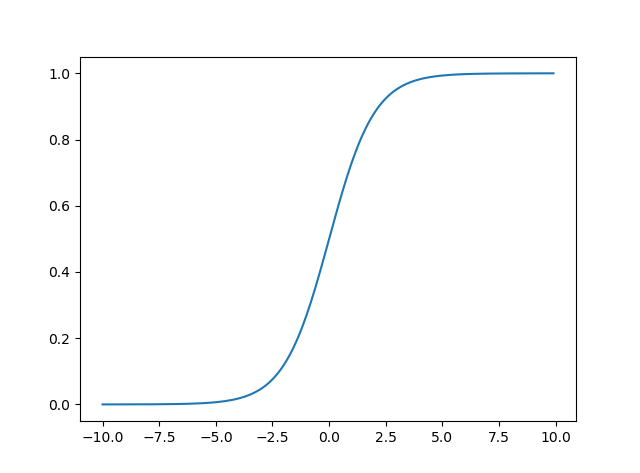
\includegraphics[scale=0.5]{../figures/NN3.png} 
\end{center}
sigmoid激活函数考虑将输入值映射到$(0,1)$的区间中,该函数在定义域内连续,且导数大于0。它也有较为简单的求导结果
\begin{eqnarray}
f'(x)=f(x)(1-f(x))
\end{eqnarray}
但是在神经网络中,特别是对于层数较多的网络,通常不采用sigmoid作为激活函数,主要是因为其容易产生梯度消失的情况。当输入非常大或非常小的时候,其梯度趋近于0,反向传播的过程中直接导致梯度无法传播,无法有效地调整权重。虽然做标准化可以让数据近似服从正态分布,但梯度消失仍有可能产生,在学习过程中可能会产生输入较大或较小的情况。或许这个问题可以用batch-normalization来缓解,但明显采取一种更佳的激活函数是较为可取的做法。
\paragraph{ReLU}
ReLU函数表达式如下
\begin{eqnarray}
f(x)=\max\{0,x\}
\end{eqnarray}
图像如下
\begin{center}
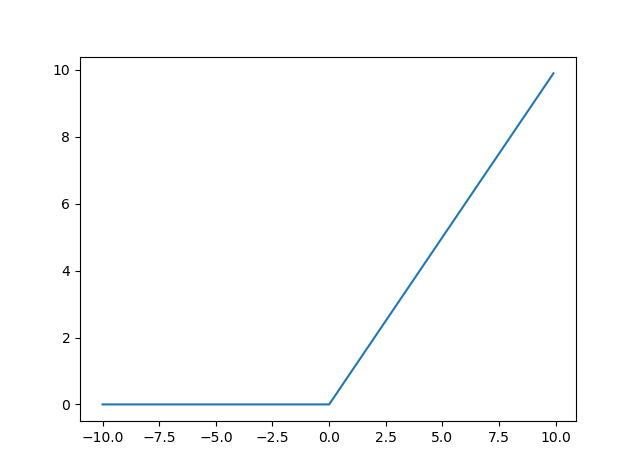
\includegraphics[scale=0.5]{../figures/NN5.png} 
\end{center}
其决定它有非常简单的求导结果
\begin{eqnarray}
f'(x)=
\left\lbrace
\begin{aligned}
1,\ x>0\\
0,\ x<0
\end{aligned}
\right.
\end{eqnarray}
RuLU收敛能比sigmoid快的多,一方面其计算快,比起sigmoid函数的导数需要指数运算,RuLU只需要做大小的比较。另一方面,其梯度经过多个层传播之后,多数能够保持原汁原味,比起sigmoid会梯度消失要好得多。然而,RuLU也有弱点,当$x<0$时$f(x)$为0,梯度为0,这直接导致该神经元失活。因而在训练过程中,要注意取较小的学习率。
\paragraph{Leaky ReLU}
Leaky ReLU是针对RuLU的弱点而改进的,其考虑用一个比较小的数去替代$x<0$时的$f(x)=0$,即
\begin{eqnarray}
f'(x)=
\left\lbrace
\begin{aligned}
x,\ x>0\\
ax,\ x<0
\end{aligned}
\right.
\end{eqnarray}
图像如下
\begin{center}
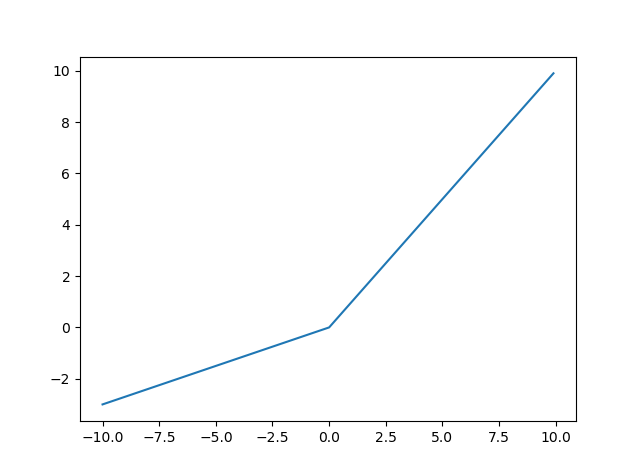
\includegraphics[scale=0.5]{../figures/NN7.png} 
\end{center}
其求导结果为
\begin{eqnarray}
f'(x)=
\left\lbrace
\begin{aligned}
1,\ x>0\\
a,\ x<0
\end{aligned}
\right.
\end{eqnarray}
这个方法可以使$x<0$处避免失活,但是额外引入了超参数$a$。
\paragraph{PReLU}PReLU是针对Leaky ReLU的进一步优化,其考虑在反向传播过程中,也对$a$进行学习,从而避免引入超参数$a$。一些实验$\ ^{[1]}$证明这种优化能取到好的学习效果。
\subsection{传统BP网络的应用}
以上介绍的BP网络的算法以及较为传统的结构,我们想探究随着图像尺寸的变化(即输入大小)以及隐含层神经元。首先我们制备数据,通过opencv的方法,将输入图像归一化为同一大小,分别为$64\times 64$,$96\times 96$,$128\times 128$,学习率设置0.03,优化函数采用Mini-batch,以8个样本作为一个batch,epoch设为600。首先考虑当隐含层分别设为1000和500时,图像大小为$64\times 64$时,模型的训练准确率如下:
\begin{center}
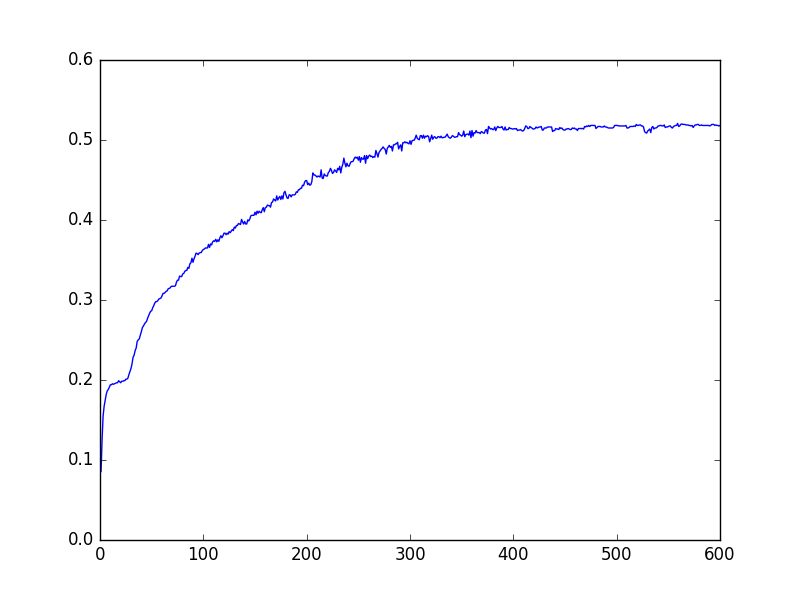
\includegraphics[scale=0.4]{../figures/Log/BP_new1/BP_new1_acc.png}
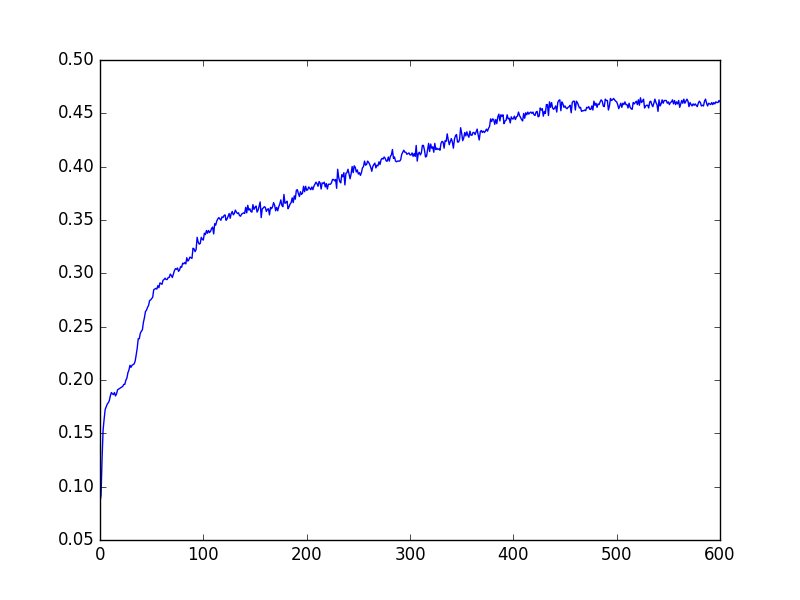
\includegraphics[scale=0.4]{../figures/Log/BP_new4/BP_new4_acc.png} \\
图像大小为$64\times 64$时,隐含层为1000和500的准确率图
\end{center}
从图中可以看出,隐含层为1000时比500好接近5\%,收敛速度上,前者在epoch为300时就趋于稳定,后者在epoch为450时趋于稳定。其原因四隐含层1000时,其自由度比500大,随着参数的增加,更有可能得到偏差小的模型。从实验可以看出,前者相比于后者在达到较低偏差的同时,其方差也不会很大。

当隐含层分别设为1000和500时,图像大小为$96\times 96$时,模型的训练准确率如下:
\begin{center}
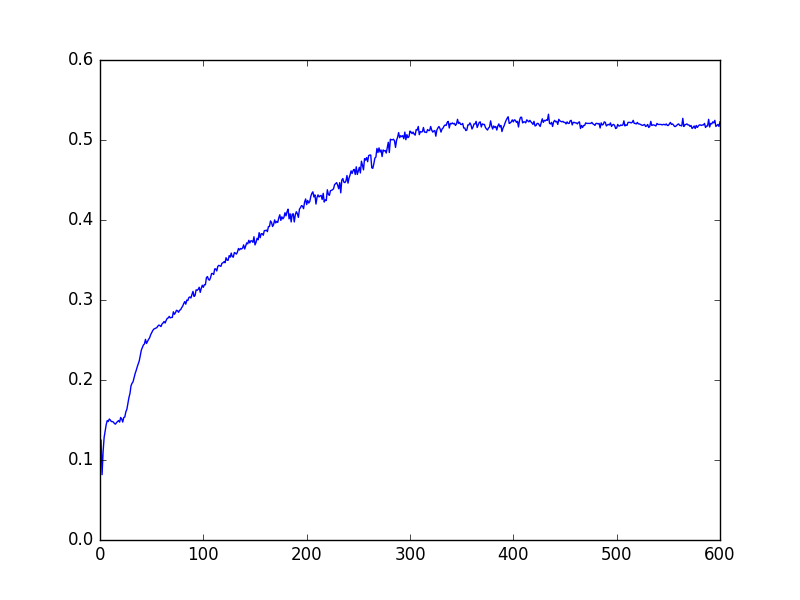
\includegraphics[scale=0.4]{../figures/Log/BP_new2/BP_new2_acc.png}
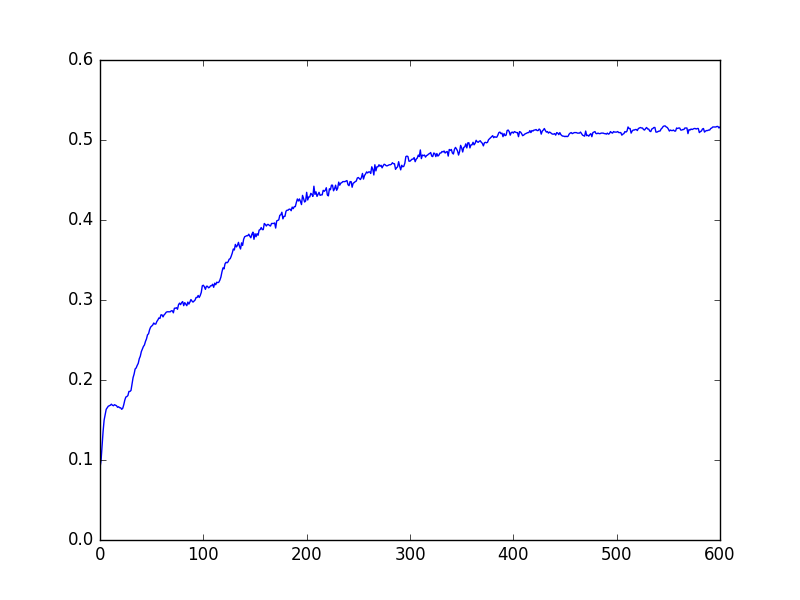
\includegraphics[scale=0.4]{../figures/Log/BP_new5/BP_new5_acc.png} \\
图像大小为$96\times 96$时,隐含层为1000和500的准确率图
\end{center}
从图中可以看出,隐含层1000与500在准确率上持平,为50\%左右。由于随着图像的尺寸增加,过拟合的风险增大。而前者相比于后者有更低的模型复杂度,一定程度上抵制了过拟合。而过拟合的风险随着图像尺寸的增大而增大的现象,我们将在下图进一步看到:

当隐含层分别设为1000和500时,图像大小为$128\times 128$时,模型的训练准确率如下:
\begin{center}
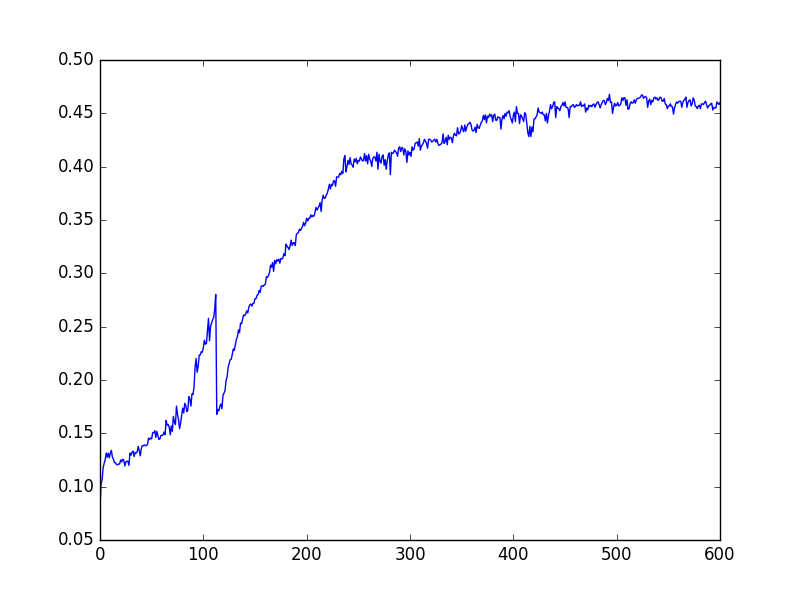
\includegraphics[scale=0.4]{../figures/Log/BP_new3/BP_new3_acc.png} 
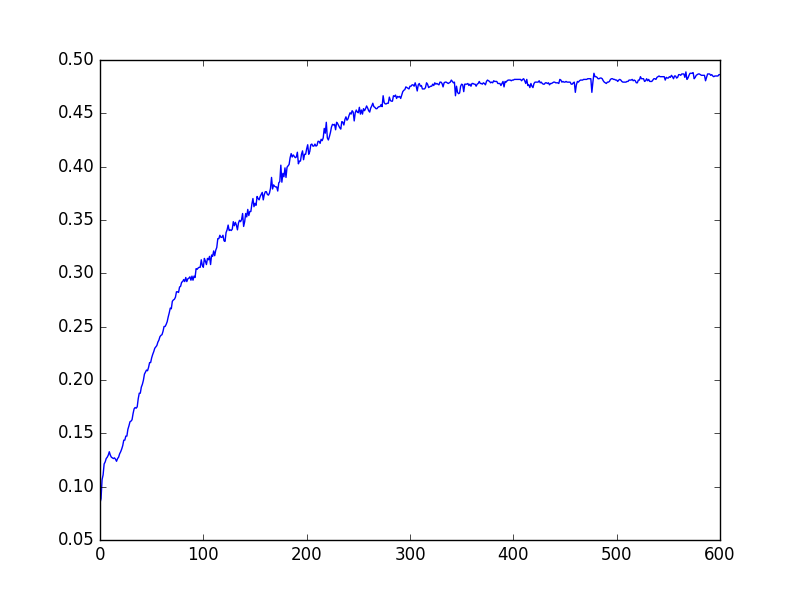
\includegraphics[scale=0.4]{../figures/Log/BP_new6/BP_new6_acc.png} \\
图像大小为$128\times 128$时,隐含层为1000和500的准确率图
\end{center}
从图中可看出,当隐含层为1000时,其训练过程中准确率出现了大幅度的震荡,而且准确率收敛在了45\%左右,而隐含层为500的模型相比隐含层为1000的模型的更加健壮,而且准确率接近50\%,比隐含层为1000的模型高了大概4\%。

综上,我们可以得到各个模型的准确率表格
\begin{center}
\begin{tabular}{cccc}
\toprule[2pt]
\  & $64\times 64$ & $96\times 96$ & $128\times 128$ \\ 
\midrule[1pt]
1000 & 0.518188 & \textbf{0.522655} & 0.460115 \\ 
500 & 0.460753 & 0.516273 & 0.48628 \\ 
\bottomrule[2pt]
\end{tabular} 
\end{center}
可以看出,在保证图像不要过大而导致过拟合下,隐含层1000的模型比隐含层500的模型性能更优。

\subsection{梯度下降方法}
梯度下降法的选取能影响收敛速度与质量,	它也是模型构成的一部分。在应用中一般有如下的梯度下降法可供选择
\paragraph{批量梯度下降法}
批量梯度下降法(Batch Gradient Descent )考虑在计算了所有样本之后再对参数进行更新,即
\begin{eqnarray}
\sample{W}{l}=\sum_{i=1}^m\sample{W}{l}-\alpha\nabla_{\sample{W}{l}}J(W,b;\sample{x}{i},\sample{y}{i})
\end{eqnarray} 
由于通常训练的样本非常大,若在计算所有样本之后再进行参数更新,会让更新的速度减慢。另外,模型实现一般会采用矩阵运算,BGD占的内存会非常多,从而影响计算速度。
\paragraph{随机梯度下降法}
随机梯度下降法(Stochastic Gradient Descent )的想法与BGD截然不同,计算每一个样本之后便进行一次反向传播,对参数进行更新,即
\begin{eqnarray}
\sample{W}{l}=\sample{W}{l}-\alpha\nabla_{\sample{W}{l}}J(W,b;x,y)
\end{eqnarray}
相比之下,SGD的训练速度比BGD快得多,在BGD进行一次反向传播的时间内,SGD已经进行过多次传播。但是在梯度下降过程中,SGD容易出现震荡,由于单个样本并不能代表梯度最大的方向,也有可能导致解非最优的情况。
\paragraph{小批量梯度下降法}
小批量梯度下降法(Mini-batch Gradient Descent )考虑了批量梯度下降法和随机梯度下降法的优缺点,并进行结合,考虑将数据集划分成多个含有较小数据的batch,然后对这些batch分别采用BGD。下面给出第$i$个batch的训练公式
\begin{eqnarray}
\sample{W}{l}=\sum_{(x,y)\in b_i}^m\sample{W}{l}-\alpha\nabla_{\sample{W}{l}}J(W,b;x,y)
\end{eqnarray}
其中,$b_i$代表当前batch所包含的训练样本$(x,y)$的集合。
\paragraph{动量梯度下降法}
无论是SGD还是MGD,即便MGD已在SGD上做了优化,在训练过程中仍可能会有振荡的风险。一种优化的方法是基于SGD,在对参数$\sample{W}{l}$进行更新时,会考虑上一次的更新幅度,若是当前的梯度方向与上一次的相同,则能够加速收敛,反之则能抑制更新,这也是采用了动量的想法。其算法如下
\begin{lstlisting}[language=python]
`输入:学习率$\epsilon$,动量参数$\alpha$`
`$t_{dW} = \alpha t_{dW} + (1-\alpha) t_{dW}$`
`$W = W - \epsilon t_{dW}$`
\end{lstlisting}
\subsection{正则化与dropout}
机器学习中,常会发生过拟合的情况,通常引起这种情况的原因有数据量过小、维度过大、模型复杂度过大等,而此现象是方差过大且偏差太小所致。通常维度过大可采用特征选择的方法来降维,而模型复杂度可以用正则化项来限制。它是考虑在损失函数中添加能反映出模型复杂度的项。例如在神经网络中,下面的损失函数的第二项称为L2正则化
\begin{eqnarray}
J(W,b;x,y) = -\sum_i y_i \log \samplet{a}{n_l}{i} + \lambda\sum_w w^2
\end{eqnarray}
我们可以把损失函数看出是由偏差衡量项(第一项)和方差衡量项(第二项)组成,其本质是偏差、方差权衡,权衡通过$\lambda$来实现。

除了L2正则化之外,常用的还有L1正则化,为如下形式
\begin{eqnarray}
J(W,b;x,y) = -\sum_i y_i \log \samplet{a}{n_l}{i} + \lambda\sum_w |w|
\end{eqnarray}

将正则化方法加入到神经网络中,设使用$96\times 96$的图像大小,隐含层神经元个数为500,学习率设置0.03,优化函数采用Mini-batch,以8个样本作为一个batch,epoch设为600。我们依次测试当正则化系数为0.1,0.01,0.001和0.0001时的模型差别,结果如下图所示
\begin{center}
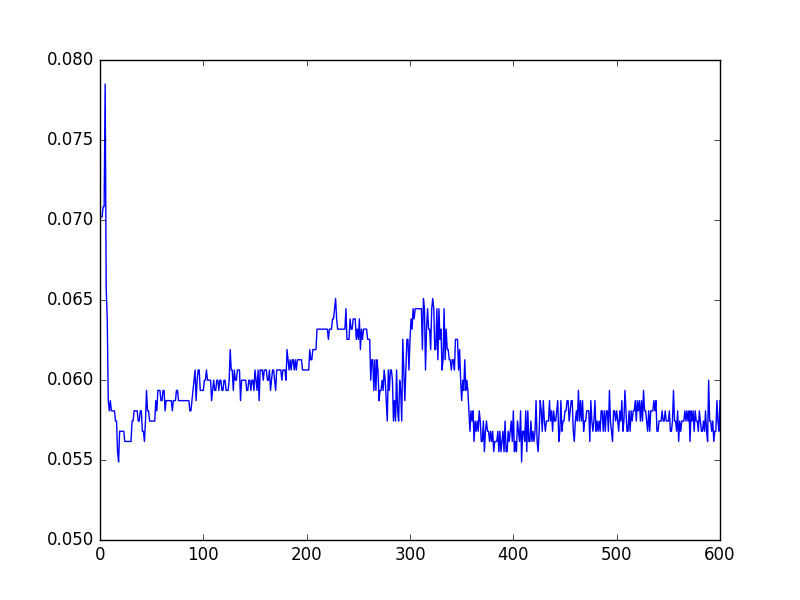
\includegraphics[scale=0.4]{../figures/Log/BP_new7/BP_new7_acc.png} 
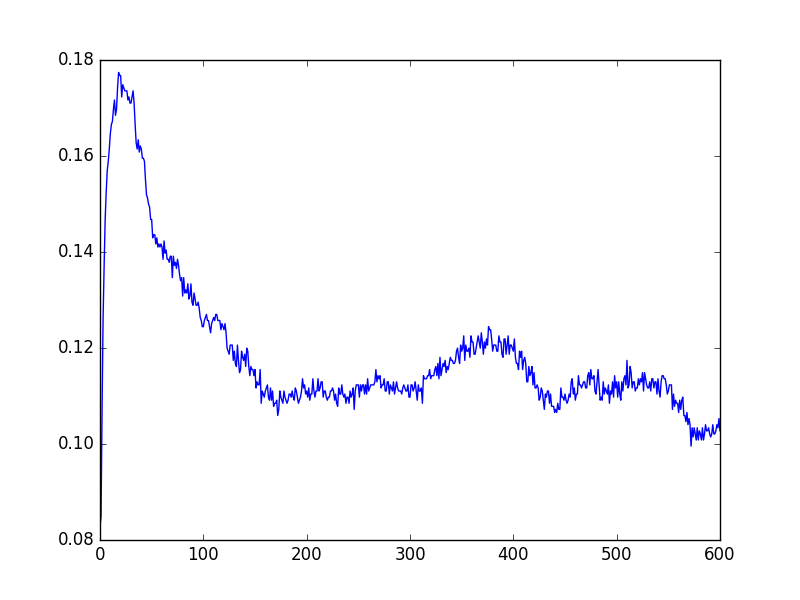
\includegraphics[scale=0.4]{../figures/Log/BP_new9/BP_new9_acc.png} \\
正则化系数为0.1和0.01
\end{center}
\begin{center}
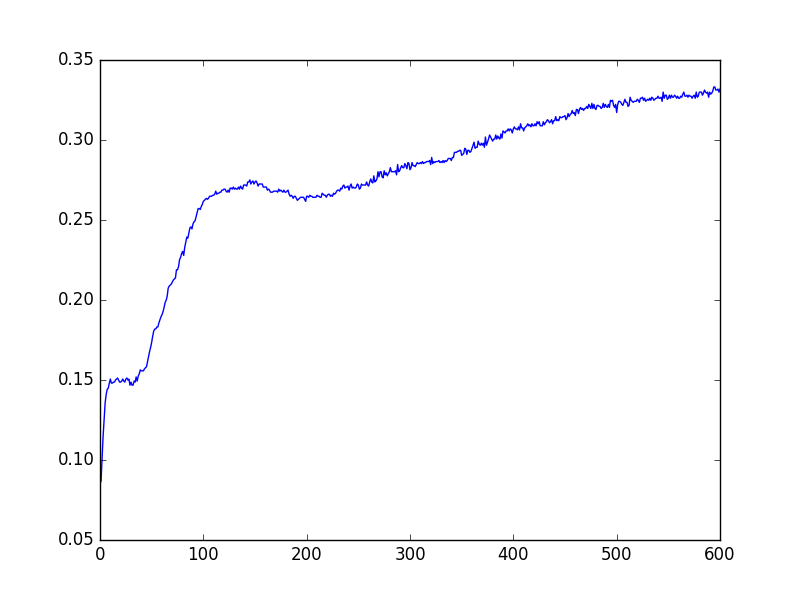
\includegraphics[scale=0.4]{../figures/Log/BP_new8/BP_new8_acc.png} 
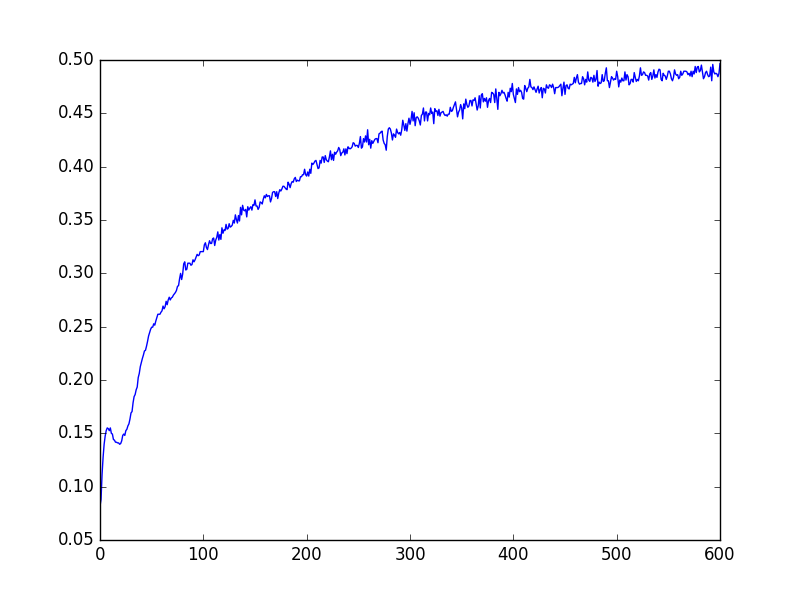
\includegraphics[scale=0.4]{../figures/Log/BP_new10/BP_new10_acc.png} \\
正则化系数为0.001和0.0001
\end{center}
其结果如下表
\begin{center}
\begin{tabular}{ccccc}
\toprule[2pt]
正则化系数 & 0.1 & 0.01 & 0.001 & 0.0001 \\ 
准确率 & 0.0587109 & 0.102744 & 0.331844 & 0.49649 \\ 
\bottomrule[2pt]
\end{tabular} 
\end{center}
可以看出,只有一层隐含层的BP网络对于正则化系数很敏感。当取0.1和0.01时,模型太过简单,以至于得不到好的模型,当放宽到0.0001时,可以解决50\%。相对而言,正则化用于复杂的模型效果会更好,例如卷积神经网络。

神经网络中,除了加入正则化项之外,还能考虑在每次训练中,让所有神经元以一定概率失活,即封闭该神经元的输出,此方法成为dropout。因而在每次训练中,网络结构都不一样,在降低模型复杂度的同时,也是对于多个模型的集成,其示意图如下。
\begin{center}
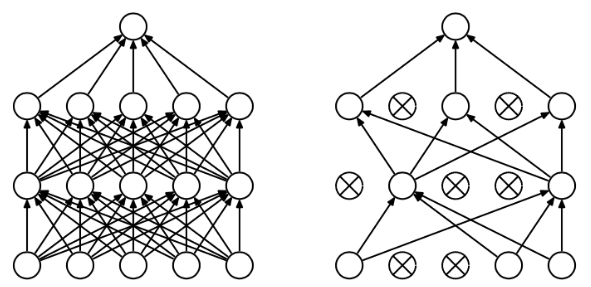
\includegraphics[scale=0.5]{../figures/dropout.png} \\
dropout工作原理示意图
\end{center}
\begin{center}
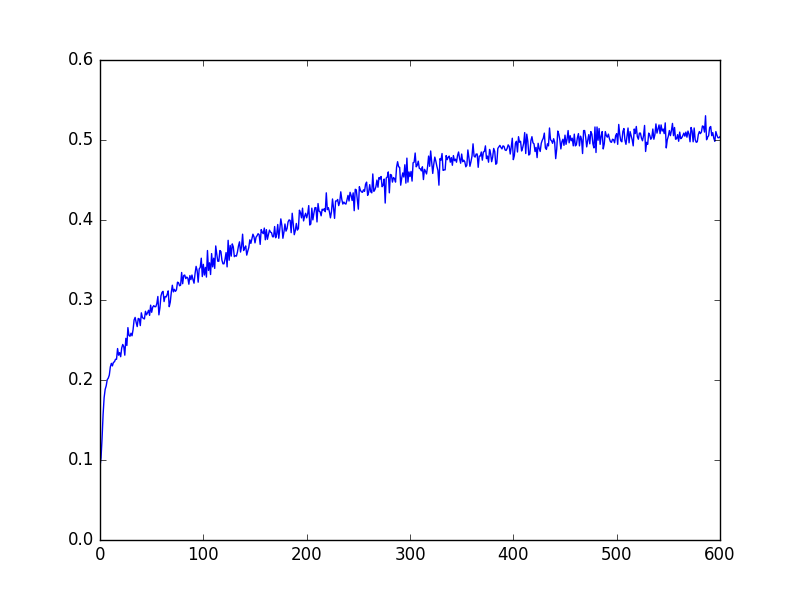
\includegraphics[scale=0.5]{../figures/Log/BP_new1_3/BP_new1_3_acc.png} \\
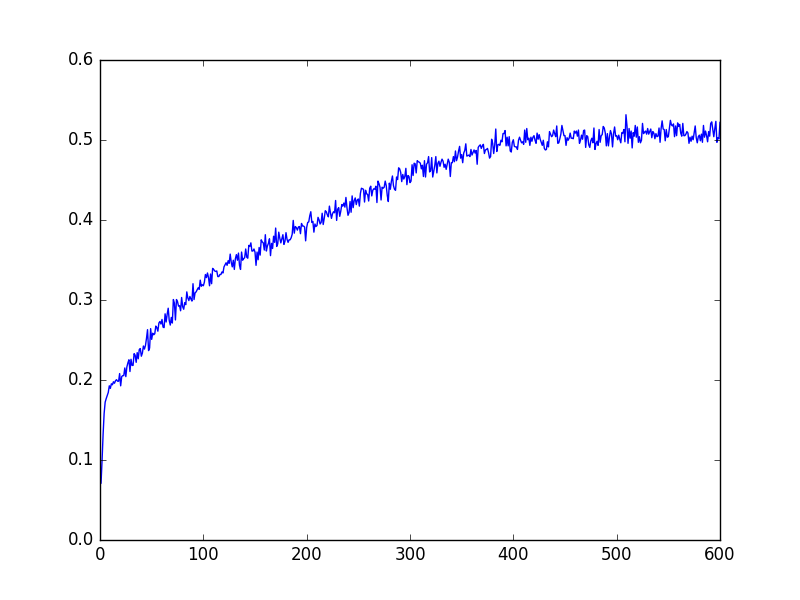
\includegraphics[scale=0.5]{../figures/Log/BP_new1_4/BP_new1_4_acc.png} 
\end{center}
\subsection{BP神经网络+X}
原始数据进行SVM的分类结果
\begin{center}
\begin{tabular}{ccccc}
\toprule[2pt]
\ & svm,linear & svm,poly & svm,rbf & svm,sigmoid \\ 
$64\times64$ & 0.361199 & 0.524569 & 0.486280 & 0.081685 \\ 
$96\times96$ & 0.388641 & 0.534142 & 0.507339 & 0.086790 \\ 
$128\times128$ & 0.373325 & 0.559668 & 0.507977 & 0.356733 \\ 
\bottomrule[2pt]
\end{tabular}
\end{center} 

由于SVM在分类问题上取得很好的效果,考虑将softmax换成SVM,有
\begin{center}
\begin{tabular}{ccccccc}
\toprule[2pt]
\ &softmax &svm,poly &nsvm,linear & nsvm,poly & nsvm,rbf & nsvm,sigmoid \\ 
$64\times64$,hid:1000 & 0.518188 & 0.524569 & 0.538609 & 0.576260 & 0.587109 & 0.081685 \\ 
$96\times96$,hid:1000 & 0.522655 & 0.534142 & 0.530951 & 0.577537 & 0.590938 & 0.075303 \\ 
$96\times96$,hid:500 & 0.516273 & 0.534142 & 0.507339 & 0.541799 & 0.580728 & 0.066369 \\ 
$96\times96$,hid:500,C=$10^{-4}$ & 0.49649 & 0.534142 & 0.529675 & 0.572431 & 0.594129 & 0.356733 \\ 
\bottomrule[2pt]
\end{tabular} 
\end{center}

为了更为直观展现结果,上表对应的条形图如下
\begin{center}
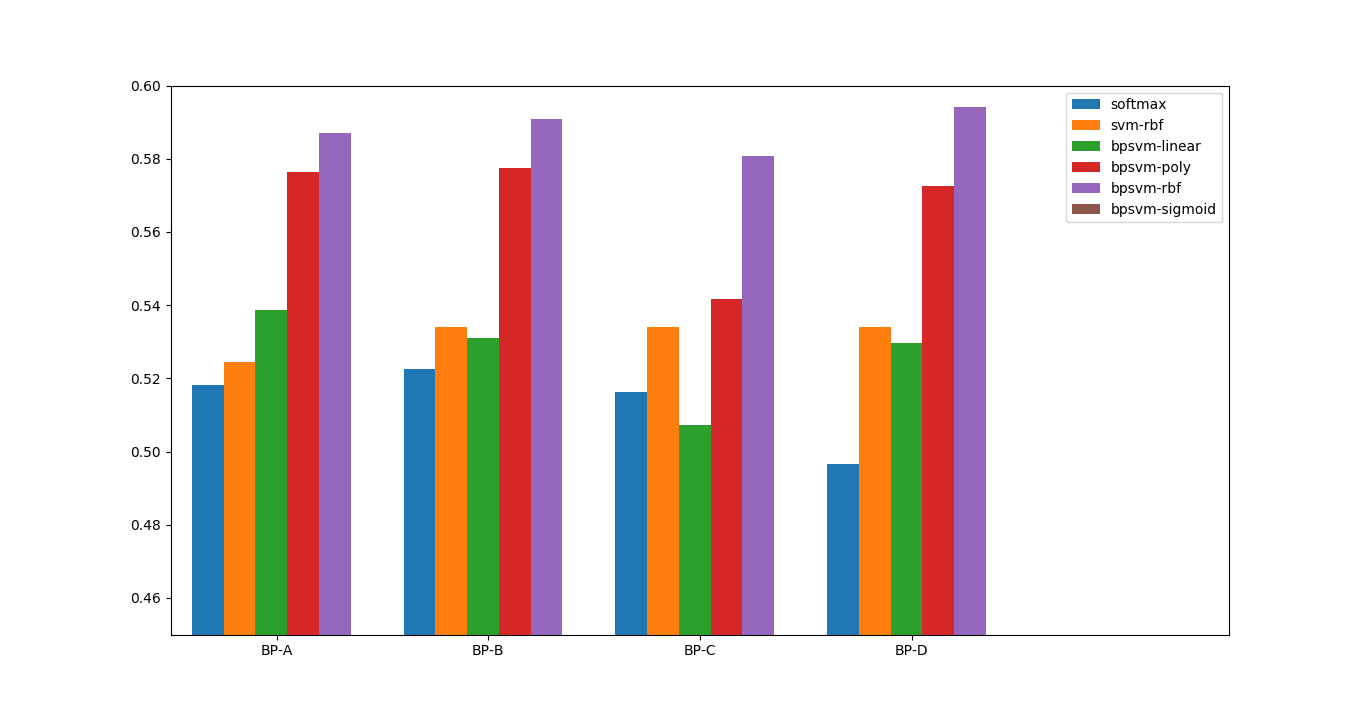
\includegraphics[scale=0.5]{../figures/NN_svm1.png} \\
BP神经网络+SVM。model A指$64\times64$,隐含层神经元个数为1000;model B指$96\times96$,隐含层神经元个数为1000;model C指$96\times96$,隐含层神经元个数为500;model D指$96\times96$,隐含层神经元个数为500,正则化系数为0.0001。
\end{center}

尝试使用决策树代替softmax,与SVM进行对比
\begin{center}
\begin{tabular}{cccccccc}
\toprule[2pt]
model  & softmax & nsvm,rbf & nCART,mdh:5 & nCART,mdh:10 & nCART,mdh:15 & nCART,mdh:20\\ 
A & 0.518188 & 0.587109 & 0.414167 & 0.417358 & 0.408424 & 0.411615\\ 
B & 0.522655 & 0.590938 & 0.416720 & 0.398851 & 0.387364 & 0.391078\\ 
C & 0.516273 & 0.580728 & 0.353542 & 0.337588 & 0.325463 & 0.327378\\ 
D & 0.49649 & 0.594129 & 0.395662 & 0.398851 & 0.389917 & 0.391193\\ 
\bottomrule[2pt]
\end{tabular} 
\end{center}


为了更为直观展现结果,上表对应的条形图如下
\begin{center}
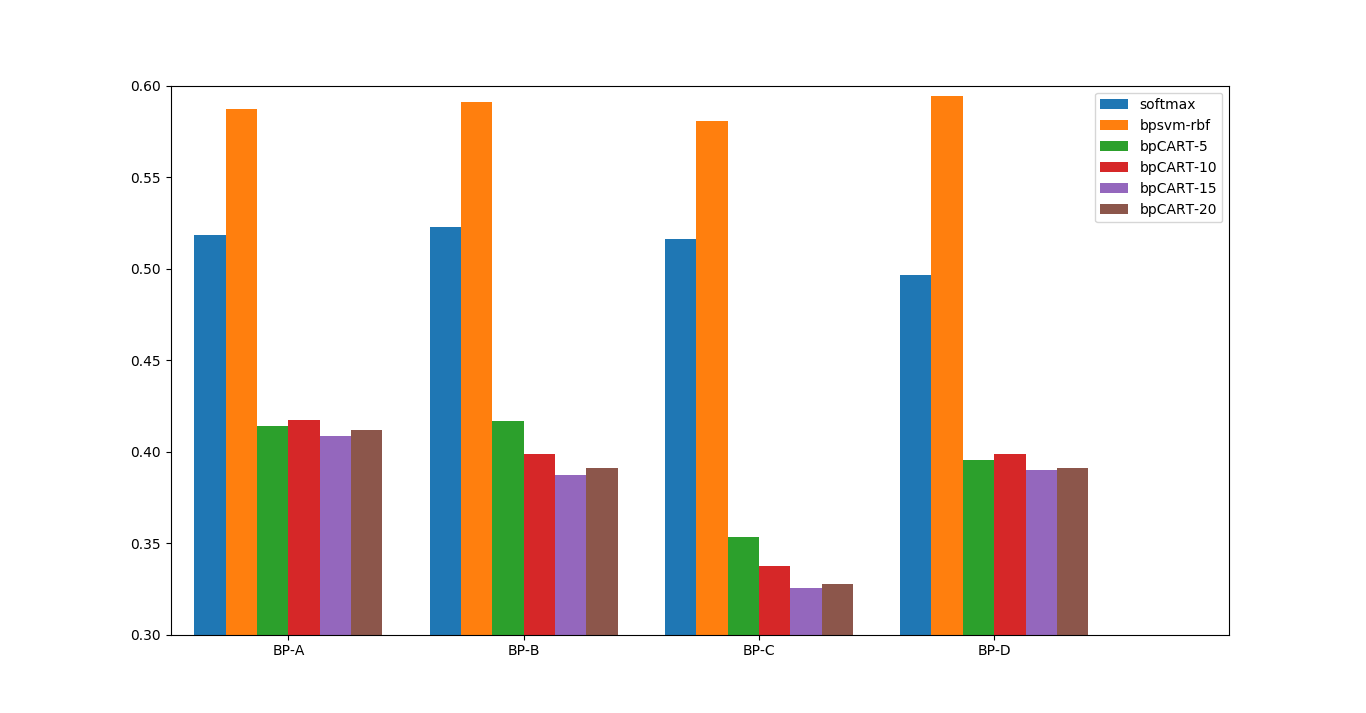
\includegraphics[scale=0.5]{../figures/NN_tree1.png} \\
BP神经网络+CART。model A指$64\times64$,隐含层神经元个数为1000;model B指$96\times96$,隐含层神经元个数为1000;model C指$96\times96$,隐含层神经元个数为500;model D指$96\times96$,隐含层神经元个数为500,正则化系数为0.0001。
\end{center}


尝试使用随机森林代替softmax,与SVM进行对比

\begin{center}
\begin{tabular}{cccccc}
\toprule[2pt]
model & softmax & nsvm,rbf & nrf,20 & nrf,50 & nrf,80 \\ 
A & 0.518188 & 0.587109 & 0.544352 & 0.552010 & 0.573070 \\ 
B & 0.522655 & 0.590938 & 0.530313 & 0.559668 & 0.574346 \\ 
C & 0.516273 & 0.5580728 & 0.504786 & 0.534780 & 0.555839 \\  
D & 0.49649 & 0.594129 & 0.523293 & 0.561583 & 0.555839 \\ 
\midrule[2pt]
model & nrf,110 & nrf,140 & nrf,170 & nrf,200 & nrf,230 \\ 
A & 0.574346 & 0.569879 & 0.577537 & 0.580089 & 0.574984 \\ 
B & 0.569879 & 0.586471 & 0.596043 & 0.583918 & 0.575622 \\ 
C & 0.545629 & 0.557754 & 0.550734 & 0.562221 & 0.569241 \\ 
D & 0.560944 & 0.573070 & 0.576899 & 0.580089 & 0.579451 \\ 
\bottomrule[2pt]
\end{tabular} 
\end{center}
\begin{center}
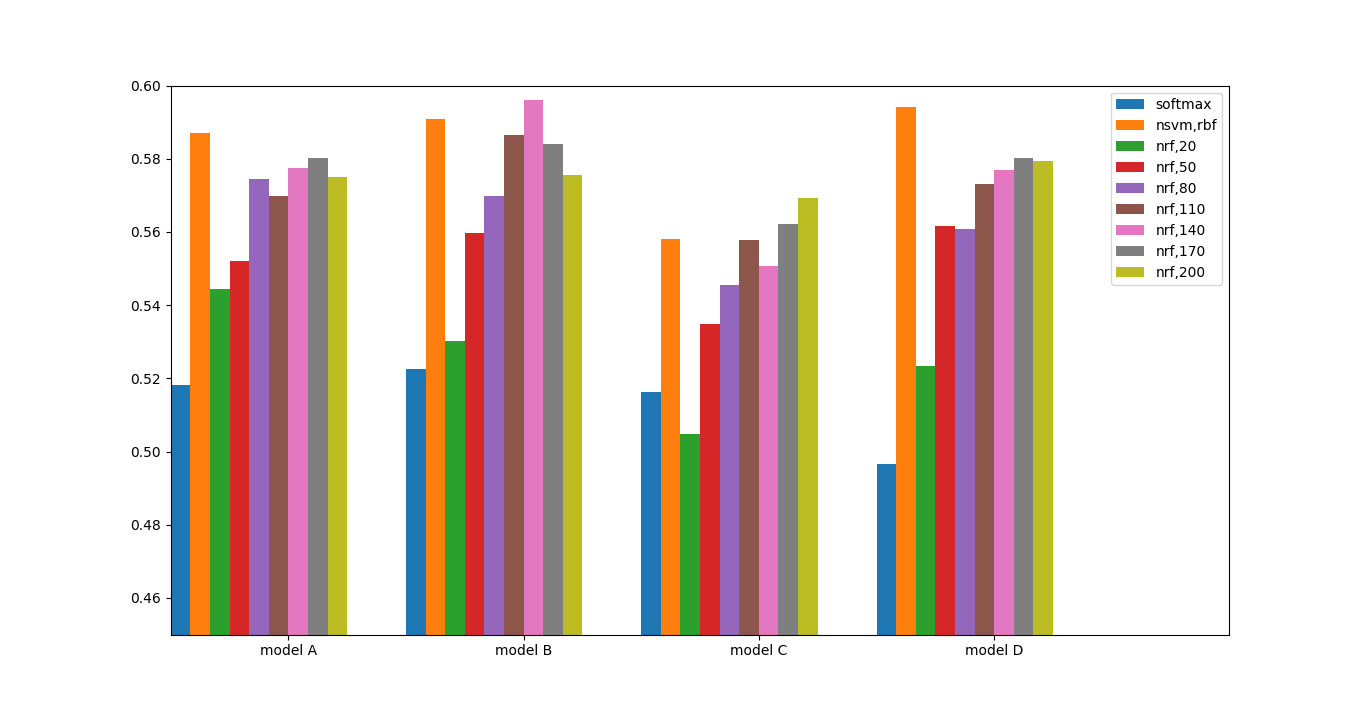
\includegraphics[scale=0.5]{../figures/NN_rf1.png} \\
BP神经网络+CART。model A指$64\times64$,隐含层神经元个数为1000;model B指$96\times96$,隐含层神经元个数为1000;model C指$96\times96$,隐含层神经元个数为500;model D指$96\times96$,隐含层神经元个数为500,正则化系数为0.0001。
\end{center}






